\documentclass{article}
\usepackage{amsmath, sfmath, multicol, tkz-euclide, array, enumerate, tcolorbox, tabularray}
\renewcommand{\familydefault}{\sfdefault}
\setlength{\parindent}{0cm}
\pagestyle{empty}
\usepackage[left=1in, top=0.5in, right=1in, bottom=0.5in]{geometry}
\tikzset{>=stealth}
\tcbset{colback=white}

\newcounter{example}[section]
\newenvironment{example}[1][]{\refstepcounter{example}\par\medskip
   {\color{red}\textbf{Example~\theexample. #1}}}{\medskip}

\begin{document}

\section*{Distance and Midpoint in the Coordinate Plane}

\begin{tcolorbox}[colframe=orange!70!white, coltitle=black, title=\textbf{Today I Can}]
\begin{enumerate}
    \item Find the distance between 2 points in the coordinate plane.
    \item Find the midpoint of a segment in the coordinate plane.
\end{enumerate}
\end{tcolorbox}

\subsection*{Distance in the Coordinate Plane}

To find the distance between 2 points in the coordinate plane, you can use the Pythagorean Theorem $a^2 + b^2 = c^2$.
\newline

\begin{example}
Find the distance between each pair of points.
\begin{enumerate}[(a)]
\begin{multicols}{2}
    \item $(5, \, 3)$ and $(-4, \, 6)$
    \item $(0, \, -6)$ and $(3, \, -1)$
\end{multicols}

\begin{tabular}{p{0.5\textwidth}p{0.5\textwidth}}
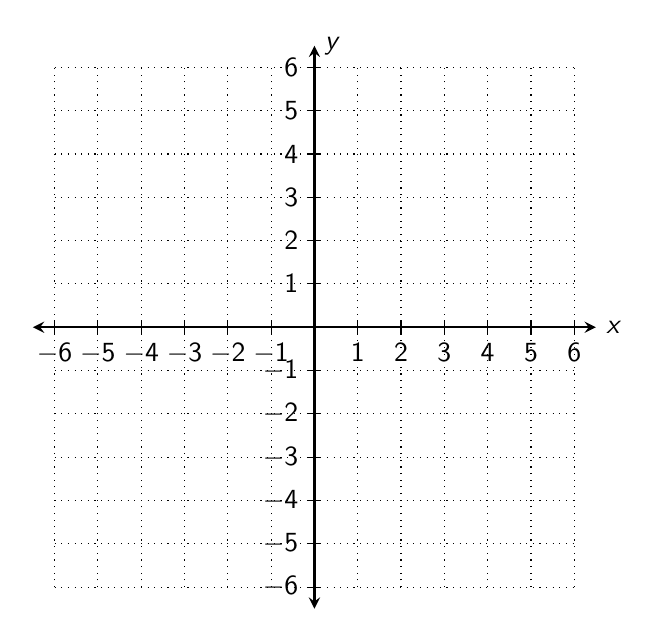
\begin{tikzpicture}[scale=0.55]
\draw[<->, thick] (-6.5,0) -- (6.5,0) node [right] {$x$};
\draw[<->, thick] (0,-6.5) -- (0,6.5) node [right] {$y$};
\draw[dotted] (-6,-6) grid (6,6);
\foreach \x in {-6,...,-1,,1,...,6}
\draw (\x, 0.15) -- (\x,-0.15) node [below] {$\tiny \x$};
\foreach \y in {-6,...,-1,,1,...,6}
\draw (0.15,\y) -- (-0.15,\y) node [left] {$\tiny \y$};
\end{tikzpicture}
&
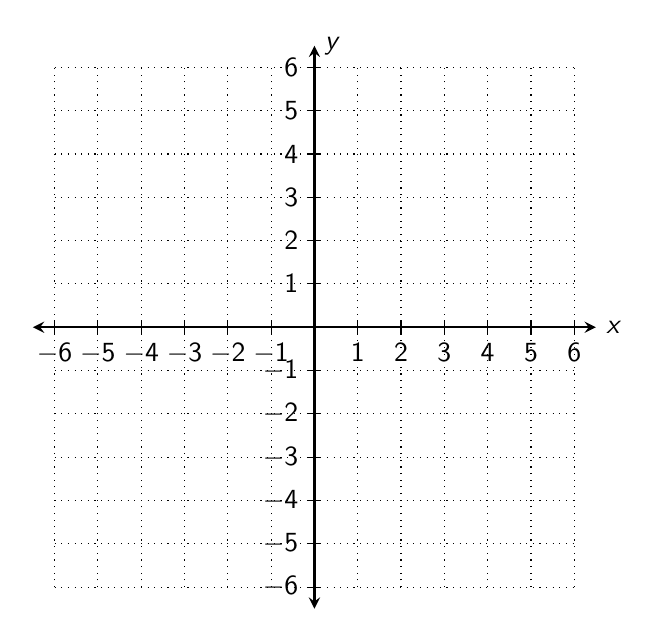
\begin{tikzpicture}[scale=0.55]
\draw[<->, thick] (-6.5,0) -- (6.5,0) node [right] {$x$};
\draw[<->, thick] (0,-6.5) -- (0,6.5) node [right] {$y$};
\draw[dotted] (-6,-6) grid (6,6);
\foreach \x in {-6,...,-1,,1,...,6}
\draw (\x, 0.15) -- (\x,-0.15) node [below] {$\tiny \x$};
\foreach \y in {-6,...,-1,,1,...,6}
\draw (0.15,\y) -- (-0.15,\y) node [left] {$\tiny \y$};
\end{tikzpicture}
\end{tabular}

\vfill 

\begin{multicols}{2}
    \item $(1, \, 5)$ and $(-2, \, 5)$
    \item $(3, 4)$ and $(3, -3)$
\end{multicols}

\begin{tabular}{p{0.5\textwidth}p{0.5\textwidth}}
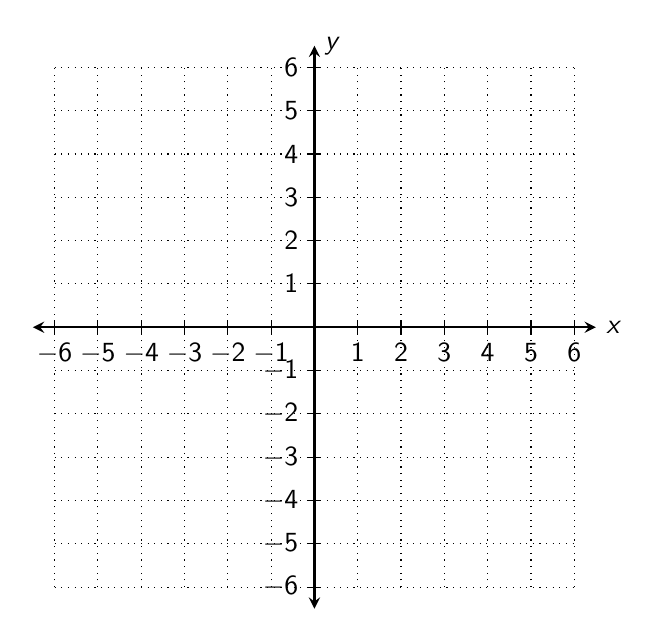
\begin{tikzpicture}[scale=0.55]
\draw[<->, thick] (-6.5,0) -- (6.5,0) node [right] {$x$};
\draw[<->, thick] (0,-6.5) -- (0,6.5) node [right] {$y$};
\draw[dotted] (-6,-6) grid (6,6);
\foreach \x in {-6,...,-1,,1,...,6}
\draw (\x, 0.15) -- (\x,-0.15) node [below] {$\tiny \x$};
\foreach \y in {-6,...,-1,,1,...,6}
\draw (0.15,\y) -- (-0.15,\y) node [left] {$\tiny \y$};
\end{tikzpicture}
&
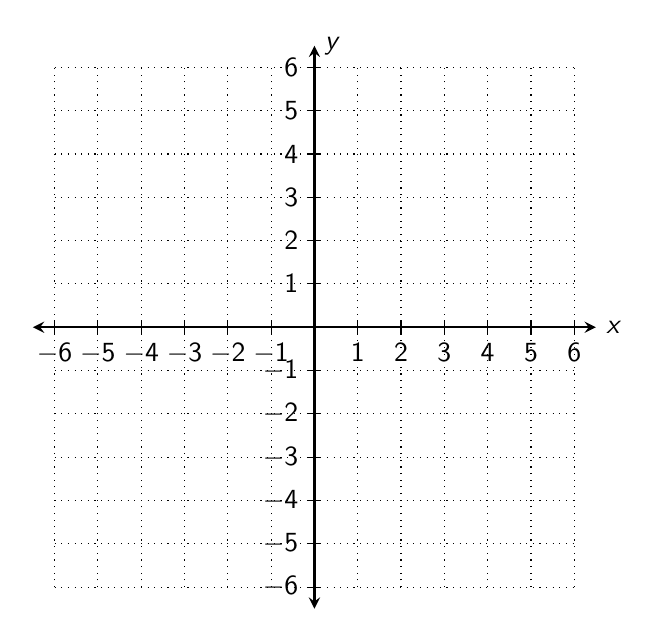
\begin{tikzpicture}[scale=0.55]
\draw[<->, thick] (-6.5,0) -- (6.5,0) node [right] {$x$};
\draw[<->, thick] (0,-6.5) -- (0,6.5) node [right] {$y$};
\draw[dotted] (-6,-6) grid (6,6);
\foreach \x in {-6,...,-1,,1,...,6}
\draw (\x, 0.15) -- (\x,-0.15) node [below] {$\tiny \x$};
\foreach \y in {-6,...,-1,,1,...,6}
\draw (0.15,\y) -- (-0.15,\y) node [left] {$\tiny \y$};
\end{tikzpicture}
\end{tabular}
\end{enumerate}
\end{example}
\vfill 

\newpage 

\subsection*{Midpoint in the Coordinate Plane}

To find the \textbf{midpoint} between 2 points, find the average of the $x$-coordinates and the average of the $y$-coordinates. \bigskip 

\begin{example}
Find the midpoint of each pair of points.
\begin{multicols}{2}
\begin{enumerate}[(a)]
    \item $(4, \, -6)$ and $(3, \, -4)$
    \item $(-5, \, 1)$ and $(-5, \, 4)$
\end{enumerate}
\end{multicols}
\begin{tabular}{p{0.5\textwidth}p{0.5\textwidth}}
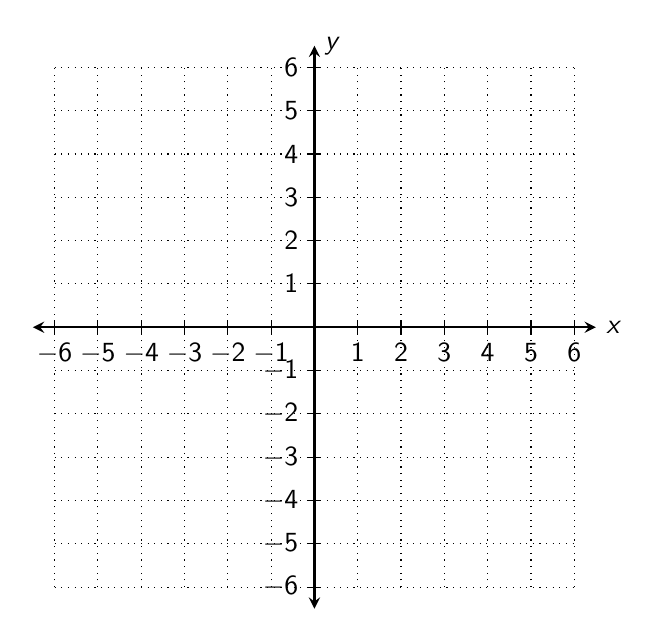
\begin{tikzpicture}[scale=0.55]
\draw[<->, thick] (-6.5,0) -- (6.5,0) node [right] {$x$};
\draw[<->, thick] (0,-6.5) -- (0,6.5) node [right] {$y$};
\draw[dotted] (-6,-6) grid (6,6);
\foreach \x in {-6,...,-1,,1,...,6}
\draw (\x, 0.15) -- (\x,-0.15) node [below] {$\tiny \x$};
\foreach \y in {-6,...,-1,,1,...,6}
\draw (0.15,\y) -- (-0.15,\y) node [left] {$\tiny \y$};
\end{tikzpicture}
&
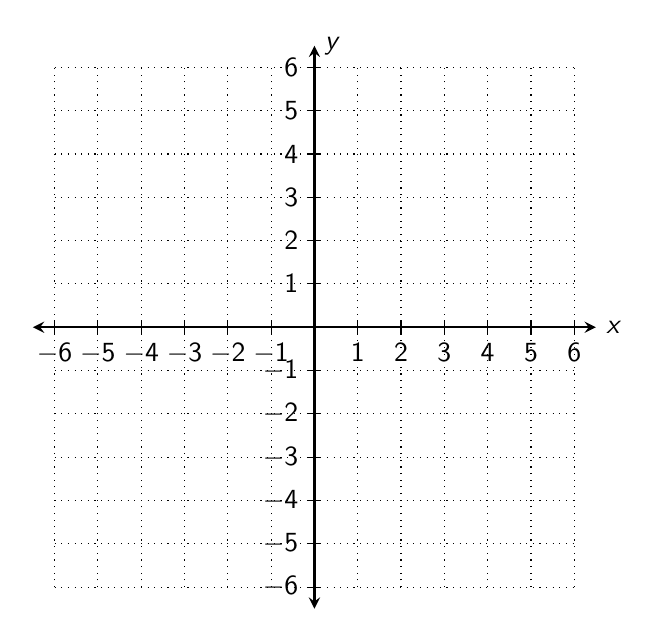
\begin{tikzpicture}[scale=0.55]
\draw[<->, thick] (-6.5,0) -- (6.5,0) node [right] {$x$};
\draw[<->, thick] (0,-6.5) -- (0,6.5) node [right] {$y$};
\draw[dotted] (-6,-6) grid (6,6);
\foreach \x in {-6,...,-1,,1,...,6}
\draw (\x, 0.15) -- (\x,-0.15) node [below] {$\tiny \x$};
\foreach \y in {-6,...,-1,,1,...,6}
\draw (0.15,\y) -- (-0.15,\y) node [left] {$\tiny \y$};
\end{tikzpicture}
\end{tabular}
\end{example}

\vfill 

\begin{example}
Find the coordinates of $B$ if $M$ is the midpoint of $\overline{AB}$.
\begin{multicols}{2}
\begin{enumerate}[(a)]
    \item $A(-2, \, -1)$;  $M(-4, \, 0)$
    \item $A(6, \, -5)$;  $M(3, \, 3)$
\end{enumerate}
\end{multicols}
\begin{tabular}{p{0.5\textwidth}p{0.5\textwidth}}
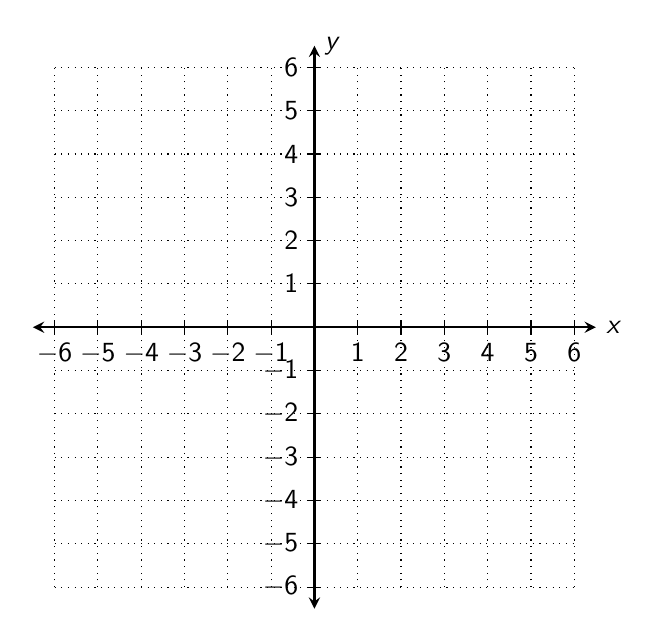
\begin{tikzpicture}[scale=0.55]
\draw[<->, thick] (-6.5,0) -- (6.5,0) node [right] {$x$};
\draw[<->, thick] (0,-6.5) -- (0,6.5) node [right] {$y$};
\draw[dotted] (-6,-6) grid (6,6);
\foreach \x in {-6,...,-1,,1,...,6}
\draw (\x, 0.15) -- (\x,-0.15) node [below] {$\tiny \x$};
\foreach \y in {-6,...,-1,,1,...,6}
\draw (0.15,\y) -- (-0.15,\y) node [left] {$\tiny \y$};
\end{tikzpicture}
&
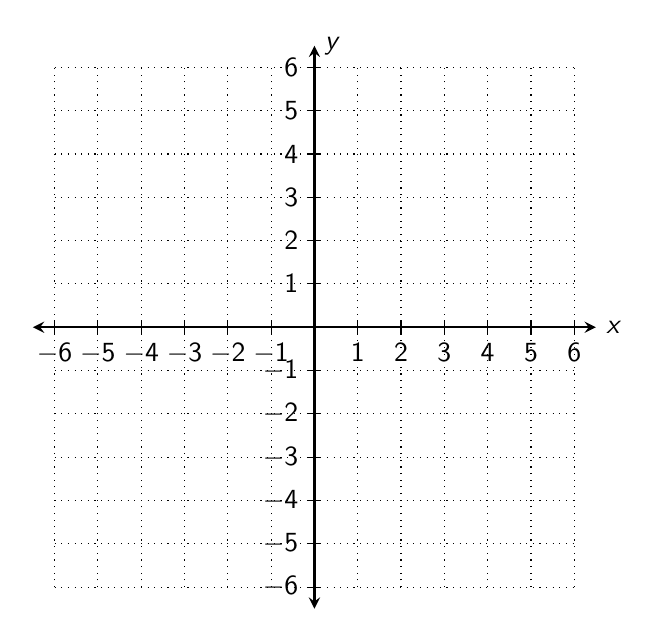
\begin{tikzpicture}[scale=0.55]
\draw[<->, thick] (-6.5,0) -- (6.5,0) node [right] {$x$};
\draw[<->, thick] (0,-6.5) -- (0,6.5) node [right] {$y$};
\draw[dotted] (-6,-6) grid (6,6);
\foreach \x in {-6,...,-1,,1,...,6}
\draw (\x, 0.15) -- (\x,-0.15) node [below] {$\tiny \x$};
\foreach \y in {-6,...,-1,,1,...,6}
\draw (0.15,\y) -- (-0.15,\y) node [left] {$\tiny \y$};
\end{tikzpicture}
\end{tabular}
\end{example}

\vfill 

\end{document}
